\documentclass[a4paper, 12pt]{article}

\usepackage[utf8]{inputenc}
\usepackage{tikz}
\include{lenguajejs.tex}
\usetikzlibrary{automata}
\usepackage{listings}
\usepackage[a4paper,bindingoffset=0.2in,%
            left=1in,right=1in,top=1in,bottom=1in,%
            footskip=.25in]{geometry}
\title{Memoria de la Práctica de Procesadores de Lenguajes: Analizador Léxico}
\author{Diego José Abengózar Vilar, Alejandro García Castellanos,\\ Ignacio Javier Encinas Ramos\\\\Grupo 82}

\renewcommand*\contentsname{Índice}

\begin{document}
\maketitle
\tableofcontents
\newpage

\section{Diseño del Analizador Léxico}

\subsection{Tokens}
\indent

$<$PuntoComa, - $>$

$<$CorcheteAbrir, - $>$ 

$<$CorcheteCerrar, - $>$

$<$ID, posTS$>$ (Identificador)

$<$ENT, valor$>$ (Dato de tipo entero)

$<$CAD, lex$>$ (Dato de tipo cadena)

$<$ParentesisCerrar, - $>$

$<$ParentesisAbrir, - $>$

$<$SUMA, - $>$ (Operador suma)

$<$MENOR, - $>$ (Operador lógico menor)

$<$NOT, - $>$ (Operador lógico de negación)

$<$ASIG, - $>$ (Operador de asignación)

$<$ASIGOR, - $>$ (Asignación con o lógico)

$<$DEC, - $>$ (“var”)

$<$TipoVarENT, - $>$ (“int”)

$<$TipoVarLOG, - $>$ (“boolean”)

$<$TipoVarCAD, - $>$ (“string”)

$<$Print, - $>$

$<$Input, - $>$

$<$Coma, - $>$

$<$Return, -$>$

$<$DECFunc, - $>$ (“function”)

$<$IF, - $>$

$<$ELSE, - $>$
\subsection{Gramática}
\lstset{
  basicstyle=\itshape,
  xleftmargin=3em,
  literate={->}{$\rightarrow$}{2}
           {λ}{$\lambda$}{1}
}

\begin{lstlisting}
G(N, T, S, P)

S = A
N = { A, B, C, D, E, F, G, H }
T = { del, ;, {, }, (, ), +, <, !, =, ,, l, d, ', /, _, *, c }   

P:
A -> delA | ; | { | } | ( | ) | + | < | ! | = | ,
A -> B | lC | dD | 'E | /F
B -> =
C -> lC | dD | _C | λ
D -> dD | λ
E -> cE | *E | /E | '
F -> *G
G -> cG | /G | *H
H -> /A | cG | *H
Donde, c = T - {*, /}
\end{lstlisting}

\subsection{Autómata Finito Determinista}
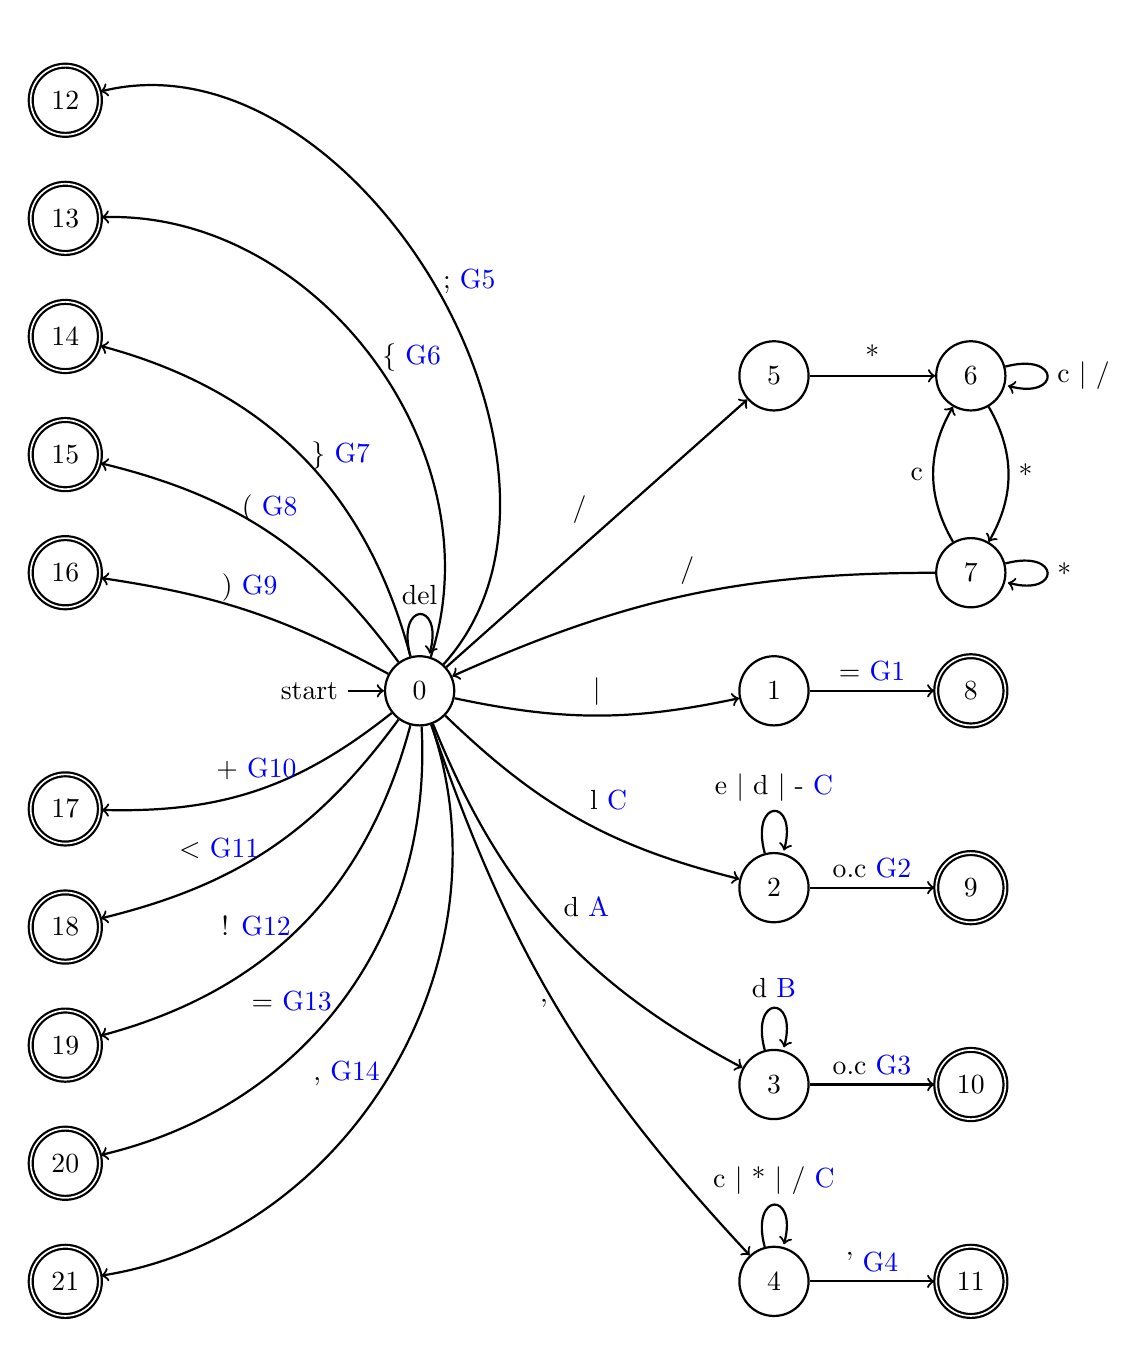
\begin{tikzpicture}[->,thick, node distance= 2.5cm,auto]
\tikzstyle{nodoChiquito} = [state, accepting, node distance = 1.5cm];
\node [state, initial](0){$0$};

\node [state](1)[right of = 0, xshift=2cm]{$1$};
\node [state, accepting](8)[right of = 1]{$8$};

\node [state](5)[above of = 1,yshift=1.5cm]{$5$};
\node [state](6)[right of = 5]{$6$};
\node [state](7)[below of = 6]{$7$};

\node [state](2)[below of = 1]{$2$};
\node [state, accepting](9)[right of = 2]{$9$};

\node [state](3)[below of = 2,]{$3$};
\node [state, accepting](10)[right of = 3]{$10$};

\node [state](4)[below of = 3]{$4$};
\node [state, accepting](11)[right of = 4]{$11$};

\node [nodoChiquito](12)[left of = 0,yshift=7.5cm,xshift=-3cm]{$12$};
\node [nodoChiquito](13)[below of = 12]{$13$};
\node [nodoChiquito](14)[below of = 13]{$14$};
\node [nodoChiquito](15)[below of = 14]{$15$};
\node [nodoChiquito](16)[below of = 15]{$16$};
\node [nodoChiquito](17)[below of = 16,yshift=-1.5cm]{$17$};
\node [nodoChiquito](18)[below of = 17]{$18$};
\node [nodoChiquito](19)[below of = 18]{$19$};
\node [nodoChiquito](20)[below of = 19]{$20$};
\node [nodoChiquito](21)[below of = 20]{$21$};

\path 
	(0) edge[loop above] node{del} (0)
        edge[bend right=73, right] node{; {\color{blue} G5}} (12)
        edge[bend right=55, right] node{\{ {\color{blue} G6}} (13)
        edge[bend right=30, right] node{\} {\color{blue} G7}} (14)
        edge[bend right=20, above] node{( {\color{blue} G8}} (15)
        edge[bend right=10, above] node{) {\color{blue} G9}} (16)
        edge[bend left=20, above] node{+ {\color{blue} G10}} (17)
        edge[bend left=20, left] node{$<$ {\color{blue} G11}} (18)
        edge[bend left=30, left] node{! {\color{blue} G12}} (19)
        edge[bend left=40, left] node{= {\color{blue} G13}} (20)
        edge[bend left=50, left] node{, {\color{blue} G14}} (21)
            
	    
	(0) edge [bend right=12] node{$\vert$} (1)
	(1) edge node{= {\color{blue} G1}} (8)
	
	(0) edge[bend right = 15] node{l {\color{blue} C}} (2)
	(2) edge [loop above] node{e $\vert$ d $\vert$ - {\color{blue} C} } (2)
	    edge node{o.c {\color{blue} G2}} (9)
	
	(0) edge[bend right = 20] node{d {\color{blue} A}} (3)
	(3) edge[loop above] node{d {\color{blue} B}} (3)
	    edge node{o.c {\color{blue} G3}} (10)
	    
	(0) edge[bend right=12,left] node{'} (4)
	(4) edge[loop above] node{c $\vert$ * $\vert$ / {\color{blue} C}} (4)
	    edge node{' {\color{blue} G4}} (11)
	
	(0) edge node{/} (5)
	(5) edge node{*} (6)
	(6) edge [bend left] node{*} (7)
	    edge [loop right] node{c $\vert$ /} (6)
	(7) edge [bend left] node {c} (6)
	    edge [loop right] node{*} (7)
	    edge[bend right=12, above] node {/} (0)
;
\end{tikzpicture}
\newpage
\subsection{Acciones Semánticas}
\lstset{
  basicstyle=\mdseries,
  xleftmargin=3em,
  mathescape=true
}

\begin{lstlisting}
Lee $\forall$ transicion menos o.c

C:  CONCAT()

$G_1$:  GEN_TOKEN(ASIGOR, -)

$G_2$: if(lex $\in$ palRes) GEN_TOKEN(palRes, -)
else if(FlagDeclUso = Decl)
	if (estaEnTSActual(lex)) 
		Error("Variable ya declarada")
	else 
		p = INSERTAR_TS(lex)
		GEN_TOKEN(ID, p)
else 
	p = BUSCA_TS(lex)
	if (p = null) p = INSERTAR_TS(lex)
	GEN_TOKEN(ID, p)

A: num = valor(d)

B: num = num * 10 + valor(d)

$G_3$: if(num $>=$ $2^{15}$) Error("Numero se sale del rango")
    else GEN_TOKEN(ENT, num)

$G_4:$ GEN_TOKEN(CAD, lex)

$G_5:$ GEN_TOKEN(PuntoComa, -)

$G_6:$ GEN_TOKEN(CorcheteAbrir, -)

$G_7:$ GEN_TOKEN(CorcheteCerrar, -)

$G_8:$ GEN_TOKEN(ParentesisAbrir, -)

$G_9:$ GEN_TOKEN(ParentesisCerrar, -)

$G_{10}:$ GEN_TOKEN(SUMA, -)

$G_{11}:$ GEN_TOKEN(MENOR, -)

$G_{12}:$ GEN_TOKEN(NOT, -)

$G_{13}:$ GEN_TOKEN(ASIG, -)

$G_{14}:$ GEN_TOKEN(Coma, -)	
\end{lstlisting}
Donde, palRes $=$ $\{$var, int, boolean, string, print, input, function, return, if, else$\}$
\newline

\subsection{Errores}
Los errores que pueden ocurrir son errores de transiciones imprevistas, error de que un número esté fuera de rango y error de identificador ya declarado previamente (cuando el FlagDeclUso= DECL).

\subsection{Matriz de Transiciones}
\hspace*{-50pt}\setlength{\tabcolsep}{0.7\tabcolsep} \begin{tabular}{|c|c|c|c|c|c|c|c|c|c|}
\hline
    \textbf{MT\_AFD} & \textbf{\textbar}  & \textbf{letra} & \textbf{digito} & \textbf{'}     & \textbf{/}     & \textbf{\_}    & \textbf{carácter} & \textbf{*}     & \textbf{delimitador} \\
\hline
 $\rightarrow$ 0     & 1 lee & 2 C   & 3A    & 4 lee & 5 lee & -1 error & -1 error & -1 error & 0 lee \\
\hline
    1     & -1 error & -1 error & -1 error & -1 error & -1 error & -1 error & -1 error & -1 error & -1 error \\
\hline
    2     & 9 G2  & 2 C   & 2 C   & 9 G2  & 9 G2  & 2 C   & 9 G2  & 9 G2  & 9 G2 \\
\hline
    3     & 10 G3 & 10 G3 & 3 B   & 10 G3 & 10 G3 & 10 G3 & 10 G3 & 10 G3 & 10 G3 \\
\hline
    4     & 4 C   & 4 C   & 4 C   & 11 G4 & 4 C   & 4 C   & 4 C   & 4 C   & 4 C  \\
\hline
    5     & -1 error & -1 error & -1 error & -1 error & -1 error & -1 error & -1 error & 6 lee & -1 error \\
\hline
    6     & 6 lee & 6 lee & 6 lee & 6 lee & 6 lee & 6 lee & 6 lee & 7 lee & 6 lee \\
\hline
    7     & 6 lee & 6 lee & 6 lee & 6 lee & 0 lee & 6 lee & 6 lee & 7 lee & 6 lee \\
\hline
    \end{tabular}\hspace{-50pt}\\\\

\hspace*{-70pt} \begin{tabular}{|c|c|c|c|c|c|c|c|c|c|c|}
\hline
    \textbf{MT\_AFD}    & \textbf{;}  & \textbf{\{}     & \textbf{\}}     & \textbf{(}     & \textbf{)}     & \textbf{+}     & \textbf{\textless}     & \textbf{!}     & \textbf{=}     & \textbf{,} \\
\hline
$\rightarrow$ 0 & 12 G5 & 13 G6 & 14 G7 & 15 G8 & 16 G9 & 17 G10 & 18 G11 & 19 G12 & 20 G13 & 21 G14 \\
\hline
    1  & -1 error & -1 error & -1 error & -1 error & -1 error & -1 error & -1 error & -1 error & 8 G1  & -1 error \\
\hline
    2 & 9 G2 & 9 G2  & 9 G2  & 9 G2  & 9 G2  & 9 G2  & 9 G2  & 9 G2  & 9 G2  & 9 G2 \\
\hline
    3 & 10 G3 & 10 G3 & 10 G3 & 10 G3 & 10 G3 & 10 G3 & 10 G3 & 10 G3 & 10 G3 & 10 G3 \\
\hline
    4 & 4 C & 4 C   & 4 C   & 4 C   & 4 C   & 4 C   & 4 C   & 4 C   & 4 C   & 4 C \\
\hline
    5 & -1 error & -1 error & -1 error & -1 error & -1 error & -1 error & -1 error & -1 error & -1 error & -1 error \\
\hline
    6 & 6 lee & 6 lee & 6 lee & 6 lee & 6 lee & 6 lee & 6 lee & 6 lee & 6 lee & 6 lee \\
\hline
    7 & 6 lee & 6 lee & 6 lee & 6 lee & 6 lee & 6 lee & 6 lee & 6 lee & 6 lee & 6 lee \\
\hline
    \end{tabular}\hspace{-70pt}

    
\section{Tabla de Símbolos: Estructura e implementación}
Contiene la información de los identificadores, de los cuales se guardan los campos: lexema, tipo y desplazamiento.
Para las funciones, además, se guardará el número de parámetros, su tipo, la forma de paso de parámetros y el tipo del valor de retorno.

La tabla de símbolos estará formada por dos matrices de tamaño dinámico; la primera contendran los indentificadores de ámbito global y la segunda del local. Así pues, esta segunda se creará al encontrar la declaración de una función y se borrará al acabar de ser declarada. También se utiliza un flag de declaración o uso (FlagDeclUso), un flag para saber cual es la tabla actual y dos más para el valor del desplazamiento en cada una de las tablas.

Sin embargo, en la implementación actual sólo se usa una tabla y siempre se supone que está el FlagDeclUso = Uso, pero en el caso de que no este declarada la variable se insertará en la tabla actual, ya que requerimos de la implementacion del Analizador Semántico para poder saber cuando se cambia de ámbito y cuando se están declarando o usando identificadores. Así que, la acción semántica que genera los tokens de los identificadores quedaría temporalmente así:
\begin{lstlisting}
$G_2$: if(lex $\in$ palRes)
	GEN_TOKEN(palRes, -)
    else if((p:= BUSCA_TS(lex))=NULL)
	p:=INSERTAR_TS(lex)
	GEN_TOKEN(ID, p)
\end{lstlisting}

\section{Anexo de Pruebas}

\textbf{Error 1: Número fuera de rango.} \\ 
\emph{Fuente}: \\
var int a; \\
var int b;\\
a = 33333;\\
b = a;\\
 if ($a  <  b$) b  =  1; \\
if ($b  <  a$) b  =  8;\\
 a = a  $+$  b;\\
print (a);\\
print (b);\medskip\\
\emph{Tokens:}\\ 
\mbox{$<$DEC, $>$}
\mbox{$<$TipoVarENT, $>$}
\mbox{$<$ID, 0$>$}
\mbox{$<$PuntoComa, $>$}
\mbox{$<$DEC, $>$}
\mbox{$<$TipoVarENT, $>$}
\mbox{$<$ID, 1$>$}
\mbox{$<$PuntoComa, $>$}
\mbox{$<$ID, 0$>$}
\mbox{$<$ASIG, $>$}\medskip\\
\emph{Tabla Simbolos:}\\
  LEXEMA: 'a'
  LEXEMA: 'b'\bigskip \\
\textbf{Error 2: Transición no prevista}\medskip\\
\emph{Fuente:} 


var string texto; /*Comentario bueno*/

 function imprime (string msg)
 
\{

	print (msg);
	
\} 

/ Comentario malo*/

function pideTexto () 

\{. 

	print ( 'Introduce un texto' ); 
	
	input (texto); 
	
\} 

 pideTexto(); 
 
var string textoAux;

textoAux = texto;

imprime (textoAux);\medskip\\
\emph{Tokens:}\\
\mbox{$<$DEC, $>$}
\mbox{$<$TipoVarCAD, $>$}
\mbox{$<$ID, 0$>$}
\mbox{$<$PuntoComa, $>$}
\mbox{$<$DECFunc, $>$} 
\mbox{$<$ID, 1$>$}

\noindent
\mbox{$<$ParentesisAbrir, $>$}
\mbox{$<$TipoVarCAD, $>$}
\mbox{$<$ID, 2$>$}
\mbox{$<$ParentesisCerrar, $>$}
\mbox{$<$CorcheteAbrir, $>$}
\mbox{$<$Print, $>$}
\mbox{$<$ParentesisAbrir, $>$}
\mbox{$<$ID, 2$>$}
\mbox{$<$ParentesisCerrar, $>$}
\mbox{$<$PuntoComa, $>$}

\noindent
\mbox{$<$CorcheteCerrar, $>$}\medskip\\
\emph{Tabla Simbolos:}\\
  LEXEMA: 'texto'
  LEXEMA: 'imprime'
  LEXEMA: 'msg'\bigskip \\
\textbf{Error 3: Transición no prevista}\\
\emph{Fuente:}

var string texto;

function pideTexto ()

\{
	print ('Introduce un texto);
	
	input (texto);
	
\}
function imprime (string msg)

\{

	print ('Mensage introducido:');
	
	print (msg);
	
\}

pideTexto();

var string textoAux;

textoAux = texto;

imprime (textoAux);\medskip\\
\emph{Tokens:}\\
 \mbox{$<$DEC, $>$} 
 \mbox{$<$TipoVarCAD, $>$ }
 \mbox{$<$ID, 0$>$ }
 \mbox{$<$PuntoComa, $>$ }
 \mbox{$<$DECFunc, $>$ }
 \mbox{$<$ID, 1$>$ }
 \mbox{$<$ParentesisAbrir, $>$ }
 \mbox{$<$ParentesisCerrar, $>$} 
 \mbox{$<$CorcheteAbrir, $>$ }
 \mbox{$<$Print, $>$ }
 
 \noindent
 \mbox{$<$ParentesisAbrir, $>$ }
 
 \noindent
$<$CAD, "\textnormal{Introduce un texto);} 
 
	input (texto);
	
\} 

\textnormal{function imprime (string msg)}

\{ 

	print (" $>$
\mbox{$<$ID, 2$>$ }
\mbox{$<$ID, 3$>$}\medskip\\
\emph{Tabla Simbolos:}\\
  LEXEMA: 'texto'
  LEXEMA: 'pideTexto'
  LEXEMA: 'Mensage'
  LEXEMA: 'introducido'\bigskip \\
\textbf{Pruebas pasadas con éxito:}\medskip\\
\textbf{1:}\smallskip\\
\emph{Fuente:} \smallskip


var int a;
 
var int b;

a = 3;

b = a;

 var boolean c;
 
c = a  $<$  b;

if (c) b  =  1;

c = b  $<$  a;

if (c) b  =  4;

 a = a  +  b;
 
print (a);

print (b);\medskip \\
\emph{Tokens:}

\smallskip
\noindent 
\mbox{$<$DEC, $>$ }
\mbox{$<$TipoVarENT, $>$} 
\mbox{$<$ID, 0$>$ }
\mbox{$<$PuntoComa, $>$} 
\mbox{$<$DEC, $>$}
\mbox{$<$TipoVarENT, $>$ }
\mbox{$<$ID, 1$>$ }
\mbox{$<$PuntoComa, $>$ }
\mbox{$<$ID, 0$>$ }
\mbox{$<$ASIG, $>$ }
\mbox{$<$ENT, 3$>$ }
\mbox{$<$PuntoComa, $>$ }
\mbox{$<$ID, 1$>$ }
\mbox{$<$ASIG, $>$ }
\mbox{$<$ID, 0$>$} 
\mbox{$<$PuntoComa, $>$ }
\mbox{$<$DEC, $>$ }
\mbox{$<$TipoVarLOG, $>$ }
\mbox{$<$ID, 2$>$ }

\noindent
\mbox{$<$PuntoComa, $>$ }
\mbox{$<$ID, 2$>$ }
\mbox{$<$ASIG, $>$ }
\mbox{$<$ID, 0$>$ }
\mbox{$<$MENOR, $>$ }
\mbox{$<$ID, 1$>$ }
\mbox{$<$PuntoComa, $>$ }
\mbox{$<$IF, $>$ }
\mbox{$<$ParentesisAbrir, $>$ }
\mbox{$<$ID, 2$>$ }
\mbox{$<$ParentesisCerrar, $>$} 
\mbox{$<$ID, 1$>$} 
\mbox{$<$ASIG, $>$ }
\mbox{$<$ENT, 1$>$ }
\mbox{$<$PuntoComa, $>$ }
\mbox{$<$ID, 2$>$ }
\mbox{$<$ASIG, $>$ }
\mbox{$<$ID, 1$>$ }
\mbox{$<$MENOR, $>$ }
\mbox{$<$ID, 0$>$ }
\mbox{$<$PuntoComa, $>$ }
\mbox{$<$IF, $>$ }
\mbox{$<$ParentesisAbrir, $>$ }
\mbox{$<$ID, 2$>$ }
\mbox{$<$ParentesisCerrar, $>$} 
\mbox{$<$ID, 1$>$ }
\mbox{$<$ASIG, $>$ }
\mbox{$<$ENT, 4$>$ }
\mbox{$<$PuntoComa, $>$} 
\mbox{$<$ID, 0$>$ }
\mbox{$<$ASIG, $>$ }
\mbox{$<$ID, 0$>$ }
\mbox{$<$SUMA, $>$ }
\mbox{$<$ID, 1$>$ }
\mbox{$<$PuntoComa, $>$ }
\mbox{$<$Print, $>$ }
\mbox{$<$ParentesisAbrir, $>$ }
\mbox{$<$ID, 0$>$ }
\mbox{$<$ParentesisCerrar, $>$ }
\mbox{$<$PuntoComa, $>$ }
\mbox{$<$Print, $>$ }
\mbox{$<$ParentesisAbrir, $>$ }
\mbox{$<$ID, 1$>$ }
\mbox{$<$ParentesisCerrar, $>$ }
\mbox{$<$PuntoComa, $>$ }\medskip\\
\emph{Tabla Simbolos:}\\ 
  LEXEMA: 'a'
  LEXEMA: 'b'
  LEXEMA: 'c'\bigskip \\
\textbf{2:}\medskip\\
\emph{Fuente:}

var int a;

var int b;

var int c;

print ( 'Introduce el primer operando' );

input (a);

print ( 'Introduce el segundo operando' );

input (b);
 
 function int suma (int num1, int num2)

\{

	return num1+num2;
	
\}

c = suma (a, b);

print (c);\medskip \\
\emph{Tokens:}

\noindent
 \mbox{$<$DEC, $>$ }
 \mbox{$<$TipoVarENT, $>$ }
 \mbox{$<$ID, 0$>$ }
 \mbox{$<$PuntoComa, $>$ }
 \mbox{$<$DEC, $>$ }
 \mbox{$<$TipoVarENT, $>$ }
 \mbox{$<$ID, 1$>$ }
 \mbox{$<$PuntoComa, $>$ }
 \mbox{$<$DEC, $>$ }
 \mbox{$<$TipoVarENT, $>$ }
 \mbox{$<$ID, 2$>$ }
 \mbox{$<$PuntoComa, $>$}
 \mbox{$<$Print, $>$ }
 \mbox{$<$ParentesisAbrir, $>$ }
 \mbox{$<$CAD, \textnormal{"Introduce el primer operando"}$>$ }
 
 \noindent
 \mbox{$<$ParentesisCerrar, $>$ }
 \mbox{$<$PuntoComa, $>$ }
 \mbox{$<$Input, $>$ }
 \mbox{$<$ParentesisAbrir, $>$ }
 \mbox{$<$ID, 0$>$ }
 \mbox{$<$ParentesisCerrar, $>$ }
 \mbox{$<$PuntoComa, $>$ }
 \mbox{$<$Print, $>$ }
 \mbox{$<$ParentesisAbrir, $>$ }
 
 \noindent
 \mbox{$<$CAD, \textnormal{"Introduce el segundo operando"}$>$ }
 \mbox{$<$ParentesisCerrar, $>$ }
 \mbox{$<$PuntoComa, $>$ }
 \mbox{$<$Input, $>$ }
 \mbox{$<$ParentesisAbrir, $>$ }
 \mbox{$<$ID, 1$>$ }
 \mbox{$<$ParentesisCerrar, $>$ }
 \mbox{$<$PuntoComa, $>$ }
 \mbox{$<$DECFunc, $>$ }
 \mbox{$<$TipoVarENT, $>$ }
 \mbox{$<$ID, 3$>$ }
 \mbox{$<$ParentesisAbrir, $>$ }
 \mbox{$<$TipoVarENT, $>$}
 \mbox{$<$ID, 4$>$ }
 \mbox{$<$Coma, $>$ }
 \mbox{$<$TipoVarENT, $>$ }
 \mbox{$<$ID, 5$>$ }
 \mbox{$<$ParentesisCerrar, $>$ }
 \mbox{$<$CorcheteAbrir, $>$ }
 \mbox{$<$Return, $>$ }
 \mbox{$<$ID, 4$>$ }
 \mbox{$<$SUMA, $>$ }
 \mbox{$<$ID, 5$>$ }
 \mbox{$<$PuntoComa, $>$ }
 \mbox{$<$CorcheteCerrar, $>$ }
 \mbox{$<$ID, 2$>$ }
 \mbox{$<$ASIG, $>$ }
 \mbox{$<$ID, 3$>$ }
 \mbox{$<$ParentesisAbrir, $>$ }
 \mbox{$<$ID, 0$>$ }
 \mbox{$<$Coma, $>$ }
 \mbox{$<$ID, 1$>$ }
 \mbox{$<$ParentesisCerrar, $>$ }
 \mbox{$<$PuntoComa, $>$ }
 \mbox{$<$Print, $>$ }
 \mbox{$<$ParentesisAbrir, $>$ }
 \mbox{$<$ID, 2$>$}
 \mbox{$<$ParentesisCerrar, $>$ }
 \mbox{$<$PuntoComa, $>$ }\medskip\\
\emph{Tabla Simbolos:}\\ 
  LEXEMA: 'a'
  LEXEMA: 'b'
  LEXEMA: 'c'
  LEXEMA: 'suma'
  LEXEMA: 'num1'
  
  \noindent
  LEXEMA: 'num2'\bigskip\\
 \textbf{3:}\medskip \\
 \emph{Fuente:}
var int a;

var int b;

a = 3;

b = a;

 if (a  $<$  b) b  =  1;
 
 a = a  +  b;
 
print (a);

print (b);
\medskip\\
\emph{Tokens:}

 \noindent
 \mbox{$<$DEC, $>$ }
 \mbox{$<$TipoVarENT, $>$ }
 \mbox{$<$ID, 0$>$ }
 \mbox{$<$PuntoComa, $>$ }
 \mbox{$<$DEC, $>$ }
 
 \noindent
 \mbox{$<$TipoVarENT, $>$ }
 \mbox{$<$ID, 1$>$ }
 \mbox{$<$PuntoComa, $>$ }
 \mbox{$<$ID, 0$>$ }
 \mbox{$<$ASIG, $>$ }
 \mbox{$<$ENT, 3$>$ }
 
 \noindent
 \mbox{$<$PuntoComa, $>$ }
 \mbox{$<$ID, 1$>$ }
 \mbox{$<$ASIG, $>$ }
 \mbox{$<$ID, 0$>$ }
 \mbox{$<$PuntoComa, $>$ }
 \mbox{$<$IF, $>$ }
 
 \noindent
 \mbox{$<$ParentesisAbrir, $>$ }
 \mbox{$<$ID, 0$>$ }
 \mbox{$<$MENOR, $>$ }
 \mbox{$<$ID, 1$>$}
 \mbox{$<$ParentesisCerrar, $>$ }
 \mbox{$<$ID, 1$>$ }
 \mbox{$<$ASIG, $>$ }
 \mbox{$<$ENT, 1$>$ }
 \mbox{$<$PuntoComa, $>$ }
 \mbox{$<$ID, 0$>$ }
 \mbox{$<$ASIG, $>$ }
 \mbox{$<$ID, 0$>$ }
 \mbox{$<$SUMA, $>$ }
 \mbox{$<$ID, 1$>$ }
 \mbox{$<$PuntoComa, $>$ }
 \mbox{$<$Print, $>$ }
 \mbox{$<$ParentesisAbrir, $>$ }
 \mbox{$<$ID, 0$>$ }
 \mbox{$<$ParentesisCerrar, $>$ }
 \mbox{$<$PuntoComa, $>$ }
 \mbox{$<$Print, $>$ }
 \mbox{$<$ParentesisAbrir, $>$ }
 \mbox{$<$ID, 1$>$ }
 \mbox{$<$ParentesisCerrar, $>$ }
 \mbox{$<$PuntoComa, $>$}\medskip\\
\emph{Tabla Simbolos:}\\ 
  LEXEMA: 'a'
  LEXEMA: 'b' 

\end{document}